\documentclass[11pt]{article}

\usepackage{amsmath}
\usepackage{amsthm}
\usepackage[spanish]{babel}
\usepackage{amssymb}
\usepackage{mathtools}
\usepackage{multirow}
\usepackage{colortbl}
\usepackage{color}
\usepackage{multicol}
\usepackage{float}
\usepackage{biblatex}
\providecommand{\N}{\mathbb{N}}
\providecommand{\Z}{\mathbb{Z}}
\providecommand{\Q}{\mathbb{Q}}
\providecommand{\R}{\mathbb{R}}
\providecommand{\C}{\mathbb{C}}
\providecommand{\H}{\mathcal{H}}
\providecommand{\Im}[1]{Im(#1)}
\providecommand{\Re}[1]{Re(#1)}
\providecommand{\conjugate}[1]{\bar{#1}}
\providecommand{\pescalar}[2]{\langle #1,#2 \rangle}
\providecommand{\braket}[2]{\left\langle#1\mid#2\right\rangle}
\providecommand{\bra}[1]{\left\langle#1\right\rvert}
\providecommand{\ket}[1]{\left\lvert#1\right\rangle}
\providecommand{\ketbra}[2]{\left\lvert#1\right\rangle\!\left\langle#2\right\rvert}
\providecommand{\avg}[1]{\left\langle#1\right\rangle}
\providecommand{\abs}[1]{\lvert#1\rvert}
\providecommand{\nor}[1]{\lVert#1\rVert}
\providecommand{\operatoravg}[3]{\left\langle#1|#2|#3\right\rangle}
\providecommand{\set}[1]{\left\{#1\right\}}
\providecommand{\so}{\Rightarrow}
\providecommand{\tq}{\mid}
\providecommand{\where}{\mathrel{}\middle|\mathrel{}}

\definecolor{unir-azul-flojo}{RGB}{230,244,249}
\definecolor{unir-azul-fuerte}{RGB}{0,152,205}
%Kets notables
\newcommand{\ketMas}{\frac{1}{\sqrt{2}}(\ket{0}+\ket{1})}
\newcommand{\ketMenos}{\frac{1}{\sqrt{2}}(\ket{0}-\ket{1})}
\newcommand{\ketIMas}{\frac{1}{\sqrt{2}}(\ket{0}+i\ket{1})}
\newcommand{\ketIMenos}{\frac{1}{\sqrt{2}}(\ket{0}-i\ket{1})}
\newcommand{\ketBellUno}{\frac{1}{\sqrt{2}}(\ket{00}+\ket{11})}
\newcommand{\ketBellDos}{\frac{1}{\sqrt{2}}(\ket{00}-\ket{11})}
\newcommand{\ketBellTres}{\frac{1}{\sqrt{2}}(\ket{10}+\ket{01})}
\newcommand{\ketBellCuatro}{\frac{1}{\sqrt{2}}(\ket{10}-\ket{01})}

%OPERADORES 2x2
\newcommand{\matrixX}{\begin{pmatrix}0 & 1 \\ 1 & 0\end{pmatrix}}
\newcommand{\matrixY}{\begin{pmatrix}0 & -i \\ i & 0\end{pmatrix}}
\newcommand{\matrixZ}{\begin{pmatrix}1 & 0 \\ 0 & -1\end{pmatrix}}
\newcommand{\matrixH}{\frac{1}{\sqrt {2}}  \begin{pmatrix}1 & 1 \\ 1 & -1\end{pmatrix}}
%OPERADORES 4x4
\newcommand{\matrixCNOT}{\begin{pmatrix}1 & 0 & 0 & 0 \\ 0 & 0 & 0 & 1 \\ 0 & 0 & 1 & 0 \\ 0 & 1 & 0 & 0\end{pmatrix}}
\usepackage[left=1.75cm,
	right=1.5cm,
	top=3.52cm,
	bottom=3.23cm]{geometry}
\usepackage{fancyhdr}
\usepackage{graphicx}
\usepackage{sectsty}
\setlength{\parskip}{\baselineskip}
\newcommand{\personalheader}[2]{
	\pagestyle{fancy}
  \setlength{\headheight}{70.866141732pt}
  \setlength{\topmargin}{-50pt}
  \setlength{\headsep}{0pt}
  \setlength{\footskip}{13.866141732pt}
	\renewcommand{\headrulewidth}{0pt}
	\fancyhead[R]{#1\\\ \\#2}
	\fancyfoot{}
	\fancyfoot[R]{\thepage}
}
\newcommand{\titulo}[1]{\textcolor{unir-azul-fuerte}{\LARGE{\textbf{#1}}}\vspace{0.1in}}
\newcommand{\primersubtitulo}[1]{\textcolor{unir-azul-fuerte}{\large #1}}
\newcommand{\subtitulo}[1]{\vspace{0.1in}\textcolor{unir-azul-fuerte}{\large #1}}
\newcommand{\seccion}[1]{\vspace{0.1in}\textbf{#1}}
\renewcommand{\labelitemi}{$\textcolor{unir-azul-fuerte}{\bullet}$}
\renewcommand{\labelitemii}{$\textcolor{unir-azul-fuerte}{\cdot}$}
\renewcommand{\labelitemiii}{$\textcolor{unir-azul-fuerte}{\diamond}$}
\renewcommand{\labelitemiv}{$\textcolor{unir-azul-fuerte}{\ast}$}
\sectionfont{\color{unir-azul-fuerte}}
\subsectionfont{\color{unir-azul-fuerte}}
\subsubsectionfont{\color{unir-azul-fuerte}}
\renewcommand*\contentsname{\textcolor{unir-azul-fuerte}{Índice de contenidos}}
\renewcommand{\listfigurename}{\textcolor{unir-azul-fuerte}{Índice de figuras}}
\renewcommand{\listtablename}{\textcolor{unir-azul-fuerte}{Índice de tablas}}
\begin{document}
	\personalheader{Nombre y apellidos del estudiante}{Título del Trabajo Fin de Estudios}
	\begin{center}
	
\includegraphics[width=10.6cm,height=2.88cm]{logo}

	\Huge Universidad Internacional de La Rioja

	\huge Escuela Superior de Ingeniería y \\ Tecnología

	\vspace{100pt}

	\LARGE Máster Universitario en Computación Cuántica

	\Huge \textcolor{unir-azul-fuerte}{Título del Trabajo Fin de Estudios}
	\normalsize

	\vspace{100pt}

\end{center}
\begin{tabular}{ll}
	Trabajo fin de estudio presentado por: & \\
	Tipo de trabajo:                       & \\
	Director/a:                            & \\
	Fecha:                                 & \\
\end{tabular}
\newpage
	\titulo{Resumen}

En este apartado se introducirá un breve resumen en español del trabajo realizado. Este resumen debe incluir el objetivo o propósito de la investigación, la metodología, los resultados y las conclusiones.

(Aproximadamente 150 palabras)

\textbf{Palabras clave:} (De 3 a 5 palabras)
	\chapter{Abstract}

En este apartado se introducirá un breve resumen en español del trabajo realizado (extensión máxima: 150 palabras). Este resumen debe incluir el objetivo o propósito de la investigación, la metodología, los resultados y las conclusiones.

{\bf Keywords:} Se deben incluir de 3 a 5 palabras claves en inglés
	\tableofcontents
\newpage
	\listoffigures
	\listoftables

	\chapter{Introducción}

El primer capítulo es siempre una introducción. En ella debes resumir de forma esquemática pero suficientemente clara lo esencial de cada una de las partes del Trabajo. La lectura de este primer capítulo ha de dar una primera idea clara de lo que se pretendía, las conclusiones a las que se ha llegado y del procedimiento seguido.

Como tal, es uno de los capítulos más importantes de la memoria. Las ideas principales a transmitir son la identificación del problema a tratar, la justificación de su importancia, los objetivos generales (a grandes rasgos) y un adelanto de la contribución que esperas hacer.

Típicamente una introducción tiene tres apartados: Motivación, Planteamiento del trabajo, Estructura del trabajo. (Texto Normal del menú de estilos.)

(Ejemplo de nota al pie\footnote{Ejemplo de nota al pie.}.)

\section{Motivación/justificación del tema a tratar}

¿Cuál es el problema que quieres tratar?

¿Cuáles crees que son las causas?

¿Por qué es relevante el problema?

A continuación, se indica con un ejemplo cómo deben introducirse los títulos y las fuentes en tablas y figuras.

\begin{table}[t]
	\begin{center}
	\caption{Ejemplo de tabla con sus principales elementos.}
	\label{tab:tab-1}
	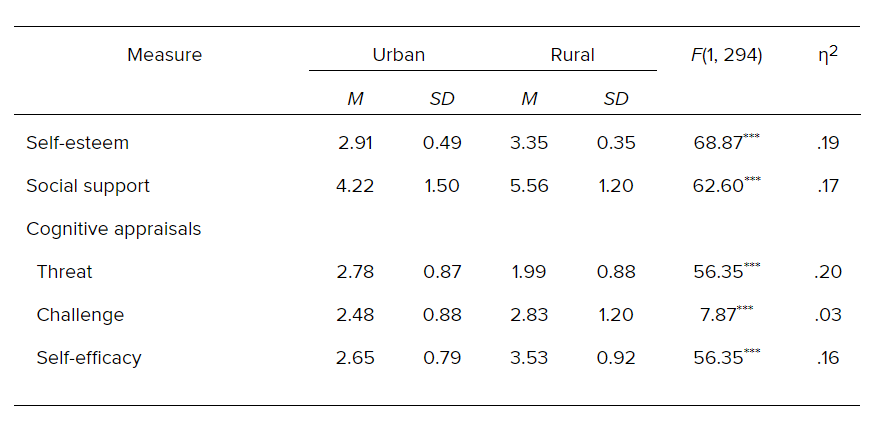
\includegraphics[width=4.90737in,height=2.42708in]{tabla}

	\small Fuente: American Psychological Association, 2020e.
	\end{center}
\end{table}

\begin{figure}[ht]
	\begin{center}
		\caption{Ejemplo de figura realizada para nuestro Trabajo.}
		\label{fig:fig-1}
		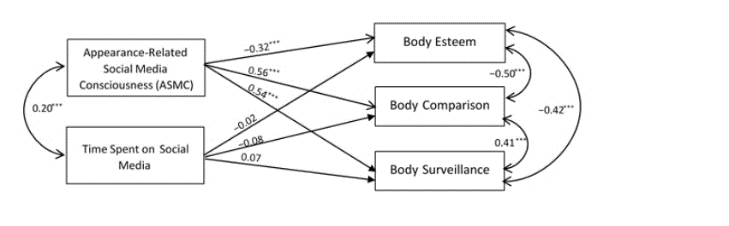
\includegraphics[width=4.90737in,height=2.42708in]{figura}

		\small Fuente: American Psychological Association, 2020f.
	\end{center}
\end{figure}

\section{Planteamiento del problema}

¿Cómo se podría solucionar el problema?

¿Qué es lo que se propone?

Aquí describes tu objetivo en términos generales.

\section{Estructura del Trabajo}

Aquí describes brevemente lo que vas a contar en cada uno de los capítulos siguientes.
	\section{Laboratorio 1: Operaciones}

	\subsection{Laboratorio 1: Operaciones}

	\section{Laboratorio 1: Operaciones}

	\subsection{Laboratorio 1: Operaciones}

	\section{Laboratorio 1: Operaciones}

	\subsection{Laboratorio 1: Operaciones}

	\section{Laboratorio 1: Operaciones}

	\subsection{Laboratorio 1: Operaciones}

	\section{Laboratorio 1: Operaciones}

	\subsection{Laboratorio 1: Operaciones}

	Para el desarrollo de los ejercicios vamos a usar las librerías qiskit, numpy y cmath:
	\newpage
	dlfsdkf
\end{document}